%% chapter01_slides.tex
%% Beamer slides for Chapter 1: Introduction
%% Algorithms for Optimization, 2nd ed. (2026)
%% Kochenderfer & Wheeler
%% Reader-friendly style: complete sentences, symbol explanations, worked examples
%% Compiled with: pdflatex -interaction=nonstopmode chapter01_slides.tex  (twice)
\documentclass[aspectratio=169,10pt]{beamer}

\usetheme{Madrid}
\usecolortheme{seahorse}

%% ── Packages ──────────────────────────────────────────────────────────────
\usepackage{amsmath,amssymb,amsfonts}
\usepackage{mathtools}
\usepackage{graphicx}
\usepackage{booktabs}
\usepackage{xcolor}
\usepackage{listings}
\usepackage{tikz}
\usepackage{pgfplots}
\pgfplotsset{compat=1.18}
\usetikzlibrary{arrows.meta,positioning,shapes.geometric,fit,backgrounds}

\graphicspath{{figures/}}

%% ── Python listing style ─────────────────────────────────────────────────
\lstdefinestyle{pycode}{
  language=Python,
  basicstyle=\ttfamily\scriptsize,
  numbers=left,
  numberstyle=\tiny\color{gray},
  frame=single,
  backgroundcolor=\color{gray!7},
  keywordstyle=\color{blue!70!black}\bfseries,
  commentstyle=\color{green!50!black}\itshape,
  stringstyle=\color{orange!80!black},
  showstringspaces=false,
  breaklines=true,
  tabsize=4,
  xleftmargin=1.5em,
  framexleftmargin=1.5em,
  aboveskip=4pt,
  belowskip=4pt,
}

%% ── Metadata ─────────────────────────────────────────────────────────────
\title[Ch.\,1 Introduction]{%
  \textbf{Chapter 1: Introduction}\\
  \normalsize Algorithms for Optimization}
\subtitle{2\textsuperscript{nd} Edition (2026)}
\author{Kochenderfer \& Wheeler}
\institute{MIT Press}
\date{2026}

\setbeamertemplate{footline}[frame number]
\setbeamertemplate{navigation symbols}{}

%% Helpful macros
\newcommand{\vx}{\mathbf{x}}
\newcommand{\R}{\mathbb{R}}
\newcommand{\grad}{\nabla}
\newcommand{\hess}{\nabla^2}

%% ══════════════════════════════════════════════════════════════════════════
\begin{document}

%% ── Title frame ──────────────────────────────────────────────────────────
\begin{frame}
  \titlepage
\end{frame}

%% ── Outline ──────────────────────────────────────────────────────────────
\begin{frame}{Chapter Overview}
  \tableofcontents
\end{frame}

\AtBeginSection[]{\begin{frame}{Outline}\tableofcontents[currentsection]\end{frame}}

%% ══════════════════════════════════════════════════════════════════════════
\section{History of Optimization}
%% ══════════════════════════════════════════════════════════════════════════

\begin{frame}[allowframebreaks]{A Brief History of Optimization}

Optimization is one of the oldest intellectual pursuits in mathematics.
Long before computers existed, thinkers were asking: ``What is the \emph{best}
arrangement, shape, or strategy?''  Understanding this history helps us see
why the mathematical tools we use today look the way they do.

  \begin{block}{Ancient Roots (300--250 BC)}
    The Greeks posed geometric extremum problems --- questions such as ``which
    shape encloses the largest area for a fixed perimeter?''  \textbf{Euclid}
    ($\sim$300 BC) established rigorous geometric reasoning, while
    \textbf{Archimedes} ($\sim$250 BC) studied the problem of maximizing the
    area of a polygon inscribed in a circle.  As the number of polygon sides
    grows without bound, the polygon area approaches the circle area --- a
    conceptual forerunner of the \emph{calculus of variations}, which optimizes
    over \emph{shapes} rather than numbers.  Much later, \textbf{Fibonacci}
    (1170--1250) popularised algebra and the idea that mathematics could be
    applied to solve practical problems of commerce and engineering.
  \end{block}

  \framebreak

  \begin{block}{The Calculus Era: 17th and 18th Centuries}
    The invention of calculus made it possible to study \emph{rates of change}
    precisely, which turns out to be exactly what is needed to find maxima and
    minima.

    \medskip
    \textbf{Fermat (1643)} observed that the derivative of a smooth function
    must equal zero at an interior maximum or minimum.  This single insight ---
    ``set the derivative to zero and solve'' --- remains the cornerstone of
    optimization theory.

    \medskip
    \textbf{Newton and Leibniz (1660s--1680s)} independently developed
    differential calculus, providing the machinery to compute derivatives
    systematically and to identify \emph{stationary points} of arbitrary
    functions.

    \medskip
    \textbf{Euler and Lagrange (1740--1770s)} extended these ideas to
    \emph{functions of functions}, founding the \emph{calculus of variations}.
    Lagrange also introduced his celebrated \emph{multiplier method} for
    handling equality constraints --- a technique still used daily in
    engineering and economics.
  \end{block}

  \framebreak

  \begin{block}{The Modern Era: Numerical and Computational Optimization}
    The 19th and 20th centuries brought two revolutions: the formalisation of
    numerical algorithms, and the arrival of computers to run them at scale.

    \medskip
    \textbf{Cauchy (1847)} proposed the \emph{steepest-descent method} ---
    the first algorithm that iteratively improves a solution by moving in the
    direction of the negative gradient.  This is the direct ancestor of every
    modern gradient-based optimizer.

    \medskip
    \textbf{Kantorovich (1939)} formulated \emph{linear programming} to solve
    production-planning problems efficiently.  His work was so influential that
    he was awarded the Nobel Prize in Economics in 1975.

    \medskip
    \textbf{Dantzig (1947)} invented the \emph{Simplex algorithm}, which made
    linear programming computationally tractable and is still widely used today.

    \medskip
    \textbf{Kuhn and Tucker (1951)} derived the \emph{KKT conditions} ---
    the necessary conditions for constrained optimality that generalise Fermat's
    derivative condition to problems with inequality and equality constraints.

    \medskip
    \textbf{The deep-learning era (2012--present)}: modern language models and
    vision systems (GPT, Llama, ResNet) are trained by minimising a loss
    function over \emph{billions} of parameters using variants of stochastic
    gradient descent.  Optimization is literally what makes AI work.
  \end{block}

  \begin{alertblock}{Key Takeaway}
    Every major advance in optimization was driven by a practical need: geometry,
    mechanics, economics, manufacturing, and now machine learning.  The algorithms
    in this book are the latest chapter in a 2000-year story.
  \end{alertblock}

\end{frame}

%% ══════════════════════════════════════════════════════════════════════════
\section{The Optimization Process}
%% ══════════════════════════════════════════════════════════════════════════

\begin{frame}[allowframebreaks]{The Optimization Process}

Optimization is not just a mathematical operation --- it is a \emph{process}
that begins with a real-world problem and ends with an implementable design.
Understanding this process prevents the common mistake of jumping straight to
an algorithm without first carefully formulating the problem.

  \begin{columns}[T]
    \column{0.48\textwidth}
      \begin{block}{The Five-Step Engineering Cycle}
        \begin{enumerate}
          \item \textbf{Specify the design problem.}  What physical or business
            system are you trying to improve?  What can you actually change
            (the \emph{design variables})?  What outcome do you care about
            (the \emph{objective})?

          \item \textbf{Choose a mathematical formulation.}  Translate the
            problem into a precise mathematical form: define the objective
            function $f(\vx)$, the design vector $\vx$, and any constraints.

          \item \textbf{Select an optimization algorithm.}  Different algorithms
            suit different problem structures.  The choice depends on the number
            of variables, whether gradients are available, and the computational
            budget.

          \item \textbf{Evaluate the design.}  Run simulations, physical
            experiments, or analytical calculations to compute $f(\vx)$ for
            candidate designs.

          \item \textbf{Iterate until convergence.}  Repeat steps 3--4,
            updating $\vx$ according to the algorithm, until improvement stalls
            or a stopping criterion is met.
        \end{enumerate}
      \end{block}

    \column{0.50\textwidth}
      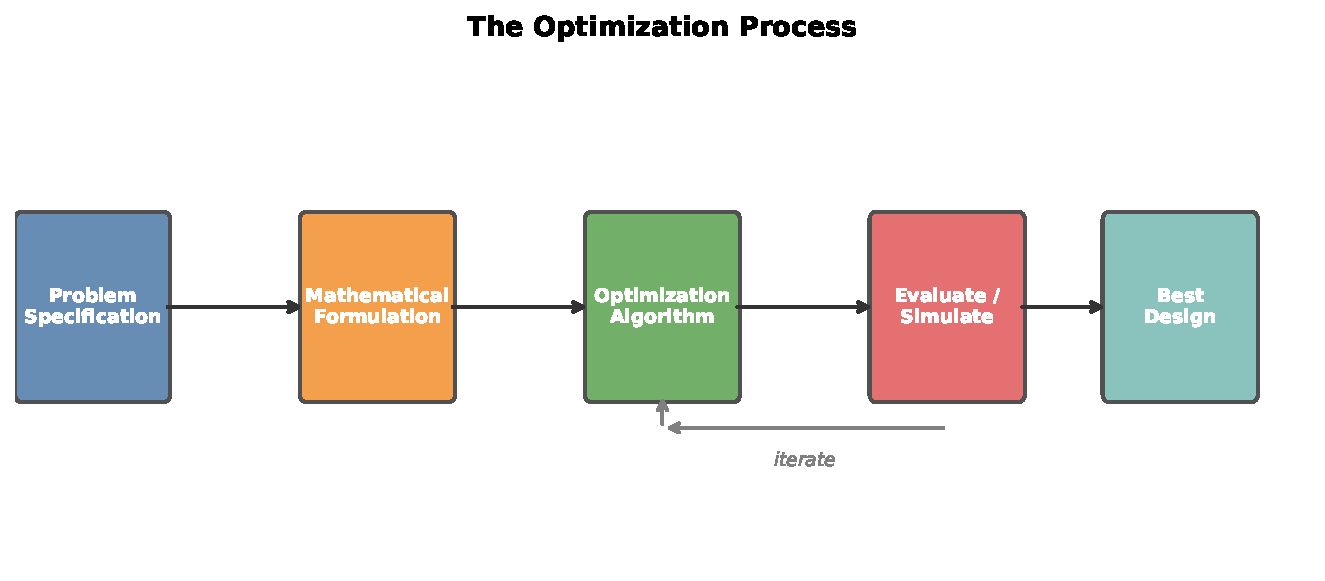
\includegraphics[width=\linewidth]{fig_opt_process}
      \vspace{0.3em}
      \begin{exampleblock}{Representative Design Problems}
        \begin{itemize}
          \item \textbf{Aerospace}: choose airfoil chord, thickness, and sweep
            angle to minimise aerodynamic drag subject to minimum-lift and
            structural-integrity constraints.
          \item \textbf{Structural engineering}: choose bicycle frame tube
            diameters to minimise mass subject to stress limits.
          \item \textbf{Control}: tune a vehicle controller's parameters to
            minimise tracking error subject to actuator limits.
          \item \textbf{Machine learning}: adjust neural network weights to
            minimise prediction error on training data.
        \end{itemize}
      \end{exampleblock}
  \end{columns}

  \framebreak

  \begin{block}{How to Choose an Algorithm}
    Before selecting an algorithm, you must characterise your problem along
    several dimensions.  There is no universally best choice --- the right
    algorithm depends on problem structure.

    \medskip
    \textbf{Dimensionality} ($n$, the number of design variables): low-dimensional
    problems ($n < 10$) allow exhaustive or derivative-free search, while
    high-dimensional problems ($n > 1000$) typically require gradient-based methods.

    \medskip
    \textbf{Gradient availability}: some problems supply exact gradients
    analytically or via automatic differentiation (Chapters 2--3); others only
    allow function evaluations (derivative-free methods, Chapter 4 onward).

    \medskip
    \textbf{Constraint structure}: unconstrained problems are simpler; bound
    constraints (Chapter 4), equality constraints, and general inequalities
    (Chapter 10) each require specialised treatment.

    \medskip
    \textbf{Evaluation budget}: if each evaluation of $f(\vx)$ requires an
    hour-long CFD simulation, you can afford far fewer iterations than if
    $f(\vx)$ evaluates in microseconds.

    \medskip
    \textbf{Noise and stochasticity}: if $f(\vx)$ is corrupted by random noise
    (e.g., measured experimentally), stochastic optimizers (Chapter 8--9) are
    more appropriate than deterministic gradient descent.

    \medskip
    \textbf{Multi-modality}: if the objective landscape has many local minima,
    global search strategies (genetic algorithms, simulated annealing, Bayesian
    optimization) may be necessary.
  \end{block}

  \begin{exampleblock}{The No-Free-Lunch Theorem (informal)}
    No single algorithm outperforms all others averaged over all possible
    problems.  This is not a counsel of despair --- it means that by
    \emph{knowing your problem structure} you can choose an algorithm that
    works well for your specific case.
  \end{exampleblock}

  \begin{block}{A Survey of Algorithm Families}
    \centering
    \begin{tabular}{lll}
      \toprule
      \textbf{Family} & \textbf{Information used} & \textbf{Representative method} \\
      \midrule
      First-order  & Gradient $\grad f$ & Gradient descent (Ch.\ 5) \\
      Second-order & Gradient + Hessian $\hess f$ & Newton's method (Ch.\ 6) \\
      Stochastic   & Noisy gradient samples & SGD, Adam (Ch.\ 8) \\
      Population   & Many function values & Genetic algorithms (Ch.\ 14) \\
      Surrogate    & Fitted model of $f$ & Bayesian optimization (Ch.\ 17) \\
      Direct search & Function values only & Nelder--Mead (Ch.\ 4) \\
      \bottomrule
    \end{tabular}
  \end{block}

\end{frame}

%% ══════════════════════════════════════════════════════════════════════════
\section{Mathematical Formulation}
%% ══════════════════════════════════════════════════════════════════════════

\begin{frame}[allowframebreaks]{Mathematical Formulation of an Optimization Problem}

Before an algorithm can be applied, the real-world problem must be translated
into a precise mathematical statement.  This section introduces the standard
form used throughout the book.

  \begin{block}{Standard Form}
    An optimization problem is written as:
    \[
      \min_{\vx \in \mathcal{X}} \; f(\vx)
      \quad \text{subject to} \quad
      g_i(\vx) \leq 0, \; i = 1,\ldots,m,
      \quad
      h_j(\vx) = 0, \; j = 1,\ldots,p
    \]
  \end{block}

  \begin{block}{Notation: Every Symbol Explained}
    \begin{itemize}
      \item $\vx = (x_1, x_2, \ldots, x_n)^\top \in \R^n$ is the
        \textbf{design vector} (also called the \emph{decision variable}).
        It is a column vector of $n$ real numbers that the algorithm is free
        to choose.  Each $x_i$ (x sub $i$) is one design parameter ---
        for example, the thickness of an airfoil at position $i$ along the wing.

      \item $f : \R^n \to \R$ is the \textbf{objective function}, a rule that
        takes a design vector $\vx$ and returns a single real number measuring
        how ``good'' that design is.  We write \emph{min} to indicate we want
        the smallest possible value.

      \item $g_i(\vx) \leq 0$ for $i = 1, \ldots, m$ are the
        \textbf{inequality constraints}.  There are $m$ (m) of them.
        Writing $g_i \leq 0$ is a convention: constraints such as
        ``thrust $\geq$ 500 N'' are rewritten as $-\text{thrust} + 500 \leq 0$.

      \item $h_j(\vx) = 0$ for $j = 1, \ldots, p$ are the
        \textbf{equality constraints}.  There are $p$ (p) of them.
        For example, ``total portfolio weight equals 1'' becomes
        $\sum_i x_i - 1 = 0$.

      \item $\mathcal{X}$ (calligraphic X, read ``script X'') is the
        \textbf{feasible set}: the set of all $\vx$ that satisfy every
        constraint simultaneously.  Only points inside $\mathcal{X}$ are
        valid solutions.
    \end{itemize}
  \end{block}

  \begin{alertblock}{How to Read This Formula}
    The expression $\min_{\vx \in \mathcal{X}} f(\vx)$ means: ``find the
    value of $\vx$ that lies inside the feasible set $\mathcal{X}$ and
    produces the smallest possible output of $f$.''  If the feasible set is
    empty (the constraints are contradictory), the problem has no solution.
    If $f$ can decrease without bound inside $\mathcal{X}$, the problem is
    \emph{unbounded} and also has no finite solution.
  \end{alertblock}

  \framebreak

  \begin{columns}[T]
    \column{0.48\textwidth}
      \begin{block}{The Feasible Set in Detail}
        The feasible set collects every design point that respects all
        constraints at once:
        \[
          \mathcal{X} = \{\,\vx \;\mid\; g_i(\vx)\leq 0 \;\forall\,i,\;
          h_j(\vx)=0 \;\forall\,j\,\}
        \]
        Here $\forall$ (for all) means ``for every.''  A point $\vx$ is called
        \textbf{feasible} when it belongs to $\mathcal{X}$, and
        \textbf{infeasible} otherwise.

        \medskip
        The feasible set can be a complicated geometric region --- a polygon,
        a curved surface, or even a disconnected collection of points.  The
        figure on the right illustrates a two-dimensional example where the
        feasible set is shaded.
      \end{block}

      \vspace{0.4em}

      \begin{block}{Three Types of Constraint}
        \begin{itemize}
          \item \textbf{Inequality}: $g(\vx) \leq 0$ --- defines a half-space
            or a curved region.
          \item \textbf{Equality}: $h(\vx) = 0$ --- restricts $\vx$ to a
            lower-dimensional surface (e.g., a plane through the origin).
          \item \textbf{Box / bound}: $l_i \leq x_i \leq u_i$ --- each variable
            is confined to a closed interval; these can be written as two
            inequality constraints.
        \end{itemize}
      \end{block}

    \column{0.50\textwidth}
      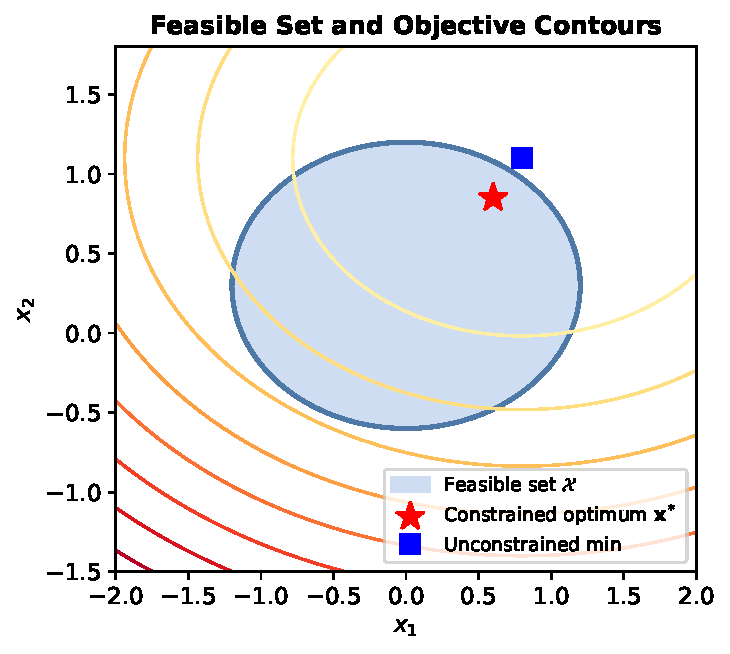
\includegraphics[width=\linewidth]{fig_feasible_set}
  \end{columns}

\end{frame}

\begin{frame}[allowframebreaks]{Feasible Set --- Worked Numerical Example}

To make the abstract formulation concrete, let us work through a small
two-dimensional example by hand.

  \begin{exampleblock}{Example: A 2-D Constrained Problem}
    We wish to minimise the squared distance from the point $(2, 1)$:
    \[
      \min_{x_1,\, x_2} \; f(x_1, x_2) = (x_1 - 2)^2 + (x_2 - 1)^2
    \]
    subject to three constraints:
    \[
      g_1:\; x_1 + x_2 \leq 2, \qquad
      g_2:\; x_1 \geq 0, \qquad
      g_3:\; x_2 \geq 0.
    \]
    Here $x_1$ (x sub 1) and $x_2$ (x sub 2) are the two decision variables.
    The objective $f$ measures the squared Euclidean distance between the
    current point $(x_1, x_2)$ and the target $(2, 1)$.
  \end{exampleblock}

  \begin{block}{Step 1: Find the Unconstrained Minimum}
    Without any constraints, we minimise $f$ by setting it to zero.
    Since $f = (x_1-2)^2 + (x_2-1)^2$ is a sum of squares, it achieves
    its minimum value of $0$ exactly at $(x_1, x_2) = (2, 1)$.

    \medskip
    \textbf{Check feasibility}: does $(2, 1)$ satisfy $g_1$?
    \[
      x_1 + x_2 = 2 + 1 = 3 \not\leq 2. \quad \text{\textcolor{red}{Infeasible!}}
    \]
    The unconstrained optimum violates the first constraint, so we cannot
    simply ignore the constraints here.
  \end{block}

  \begin{block}{Step 2: Examine Boundary Points}
    Because the unconstrained minimum is outside $\mathcal{X}$, the constrained
    minimum must lie \emph{on the boundary} of the feasible set.  We check
    the boundary $x_1 + x_2 = 2$ (where $g_1$ is active):

    \medskip
    Substituting $x_2 = 2 - x_1$ into $f$:
    \[
      f(x_1, 2-x_1) = (x_1-2)^2 + (2-x_1-1)^2 = (x_1-2)^2 + (1-x_1)^2.
    \]
    Expanding: $= x_1^2 - 4x_1 + 4 + x_1^2 - 2x_1 + 1 = 2x_1^2 - 6x_1 + 5$.
    Setting the derivative to zero: $4x_1 - 6 = 0 \Rightarrow x_1 = 1.5$.
    Then $x_2 = 2 - 1.5 = 0.5$.
    \[
      f(1.5,\, 0.5) = (1.5-2)^2 + (0.5-1)^2 = 0.25 + 0.25 = 0.5.
    \]
  \end{block}

  \begin{columns}[T]
    \column{0.55\textwidth}
      \begin{exampleblock}{Classification of Sample Points}
        \centering
        \begin{tabular}{llll}
          \toprule
          \textbf{Point} & \textbf{Feasible?} & $f$ \textbf{value} & \textbf{Note} \\
          \midrule
          $(0, 0)$   & Yes & $4 + 1 = 5$   & Corner of $\mathcal{X}$ \\
          $(1, 1)$   & Yes & $1 + 0 = 1$   & Boundary ($g_1$ active) \\
          $(1.5, 0.5)$ & Yes & $0.5$ & \textbf{Constrained optimum} \\
          $(2, 1)$   & \textcolor{red}{No}  & $0$           & Unconstrained min \\
          \bottomrule
        \end{tabular}
      \end{exampleblock}
      \begin{alertblock}{Key Insight}
        When the unconstrained minimum is infeasible, the constrained
        minimum is typically found on the \emph{boundary} of the feasible set ---
        the point closest to the unconstrained optimum that still satisfies
        all constraints.
      \end{alertblock}

    \column{0.42\textwidth}
      \begin{block}{Checking Feasibility in Python}
        A quick sanity check for any candidate point $(x_1, x_2)$:
        \begin{itemize}
          \item Compute $g_1 = x_1 + x_2 - 2$. Feasible iff $g_1 \leq 0$.
          \item Compute $g_2 = -x_1$. Feasible iff $g_2 \leq 0$, i.e.\ $x_1 \geq 0$.
          \item Compute $g_3 = -x_2$. Feasible iff $g_3 \leq 0$, i.e.\ $x_2 \geq 0$.
        \end{itemize}
        All three must hold simultaneously for the point to be in $\mathcal{X}$.
      \end{block}
  \end{columns}

\end{frame}

\begin{frame}[fragile]{Constrained Optimisation in Python --- SciPy Example}

Python's \texttt{scipy.optimize.minimize} function can solve this problem
automatically.  The code below sets up the objective, constraints, and bounds,
then calls the SLSQP solver (Sequential Least Squares Programming), which
is designed specifically for smooth constrained problems.

  \begin{columns}[T]
    \column{0.54\textwidth}
      \begin{lstlisting}[style=pycode,caption={Constrained optimization with SciPy}]
import numpy as np
from scipy.optimize import minimize

# Objective: f(x) = (x1-2)^2 + (x2-1)^2
def f(x):
    return (x[0]-2)**2 + (x[1]-1)**2

# Constraints: x1+x2 <= 2, x1>=0, x2>=0
# SciPy 'ineq' means fun(x) >= 0, so we write
# 2 - x1 - x2 >= 0  <=>  x1+x2 <= 2
constraints = [
    {'type': 'ineq', 'fun': lambda x: 2 - x[0] - x[1]},
]
# Bounds encode x1 >= 0 and x2 >= 0
bounds = [(0, None), (0, None)]

x0 = np.array([0.5, 0.5])   # initial guess
result = minimize(f, x0,
                  method='SLSQP',
                  bounds=bounds,
                  constraints=constraints)

print("Optimal x:", result.x)
print("f(x*)   :", result.fun)
# Optimal x: [1.5  0.5]
# f(x*)   : 0.5
      \end{lstlisting}

    \column{0.44\textwidth}
      \begin{block}{Reading the SciPy API}
        \begin{itemize}
          \item \texttt{method='SLSQP'}: the solver algorithm.  SLSQP handles
            both inequality and equality constraints by solving a sequence of
            quadratic subproblems.
          \item \texttt{bounds}: a list of \texttt{(lower, upper)} pairs ---
            one per variable.  \texttt{None} means no bound on that side.
          \item \texttt{constraints}: a list of dictionaries.  \texttt{'type':
            'ineq'} means $\text{fun}(\vx) \geq 0$.  Note this is the
            \emph{opposite} sign from the $g_i \leq 0$ convention: you
            may need to negate your constraint function.
          \item \texttt{result.x}: the optimal design vector $\vx^*$.
          \item \texttt{result.fun}: the optimal objective value $f(\vx^*)$.
        \end{itemize}
      \end{block}
      \begin{exampleblock}{Verifying the Output}
        The solver returns $\vx^* = (1.5,\, 0.5)$ with $f(\vx^*) = 0.5$,
        matching our hand calculation.  Checking constraint $g_1$:
        $1.5 + 0.5 = 2 \leq 2$ --- the constraint is \emph{active}
        (satisfied with equality), which confirms the solution lies on
        the boundary.
      \end{exampleblock}
  \end{columns}

\end{frame}

%% ══════════════════════════════════════════════════════════════════════════
\section{Applications}
%% ══════════════════════════════════════════════════════════════════════════

\begin{frame}[allowframebreaks]{Applications of Optimization}

Optimization pervades nearly every quantitative field.  The five examples
below show how the same mathematical framework --- choose $\vx$ to minimise
$f(\vx)$ subject to constraints --- applies across very different domains.

  \begin{columns}[T]
    \column{0.48\textwidth}

      \begin{block}{Aircraft Design (Aeronautics)}
        An aircraft designer wants to minimise aerodynamic drag $D(\vx)$,
        which directly determines fuel consumption and operating cost.
        The design vector $\vx$ collects geometric parameters of the wing
        and fuselage: chord length (the front-to-back distance of the wing),
        thickness-to-chord ratio, and sweep angle.

        \medskip
        The constraints enforce that the wing must generate at least a minimum
        amount of lift to keep the aircraft airborne, and that structural stresses
        remain below material limits.  Each function evaluation requires a
        Computational Fluid Dynamics (CFD) simulation that may take hours of
        computing time, so the optimizer must make intelligent use of a limited
        budget of evaluations.
      \end{block}

      \vspace{0.4em}

      \begin{block}{Deep Learning (Machine Learning)}
        Training a neural network means finding a weight vector $\vx \in \R^n$
        (where $n$ can be billions) that minimises the \emph{cross-entropy loss}
        $\mathcal{L}(\vx)$ measuring the discrepancy between the network's
        predictions and the true labels.  Because computing the loss over the
        entire dataset at each step is too slow, we use \emph{Stochastic
        Gradient Descent} (SGD) or Adam, which approximate the gradient using
        a random mini-batch at each iteration.
      \end{block}

    \column{0.50\textwidth}
      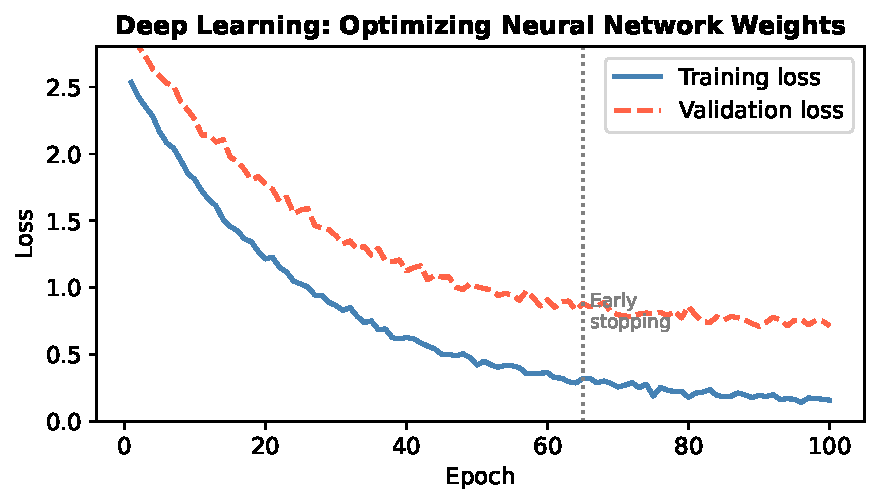
\includegraphics[width=\linewidth]{fig_dl_loss}
      \vspace{0.3em}
      \begin{block}{}
        \scriptsize The figure shows typical training and validation loss curves
        during neural-network optimization.  The training loss (solid) decreases
        monotonically as the optimizer adjusts the weights.  The validation loss
        (dashed) initially tracks the training loss, then may rise if the model
        starts to overfit --- a signal to stop training early.
      \end{block}
  \end{columns}

  \framebreak

  \begin{columns}[T]
    \column{0.48\textwidth}
      \begin{block}{Financial Portfolio Optimization (Markowitz, 1952)}
        Harry Markowitz showed that portfolio selection can be cast as a
        quadratic program.  Let $\vx \in \R^n$ be the vector of portfolio
        weights, where $x_i$ (x sub $i$) is the fraction of total wealth
        invested in asset $i$.

        \medskip
        \textbf{Objective}: minimise portfolio variance (risk) $\vx^\top
        \Sigma \vx$, where $\Sigma$ (Sigma, the covariance matrix) encodes
        how assets move together.  Simultaneously, we want the expected
        return $\boldsymbol{\mu}^\top \vx$ (where $\boldsymbol{\mu}$, mu,
        is the vector of expected returns) to exceed a target level $r_{\min}$.

        \medskip
        \textbf{Constraint}: $\sum_{i=1}^n x_i = 1$ (we must invest all
        our wealth), and $x_i \geq 0$ (no short-selling).

        \medskip
        By solving this for many values of $r_{\min}$ and plotting the
        resulting $(r_{\min},\, \sigma)$ pairs, we trace the
        \textbf{efficient frontier}: the Pareto-optimal set of
        risk--return trade-offs.
      \end{block}

      \vspace{0.3em}
      \begin{exampleblock}{Python Note}
        Use \texttt{scipy.optimize.minimize} with \texttt{method='SLSQP'},
        the equality constraint $\mathbf{1}^\top \vx = 1$ (sum of weights
        equals one), and bounds $x_i \in [0, 1]$.
      \end{exampleblock}

    \column{0.50\textwidth}
      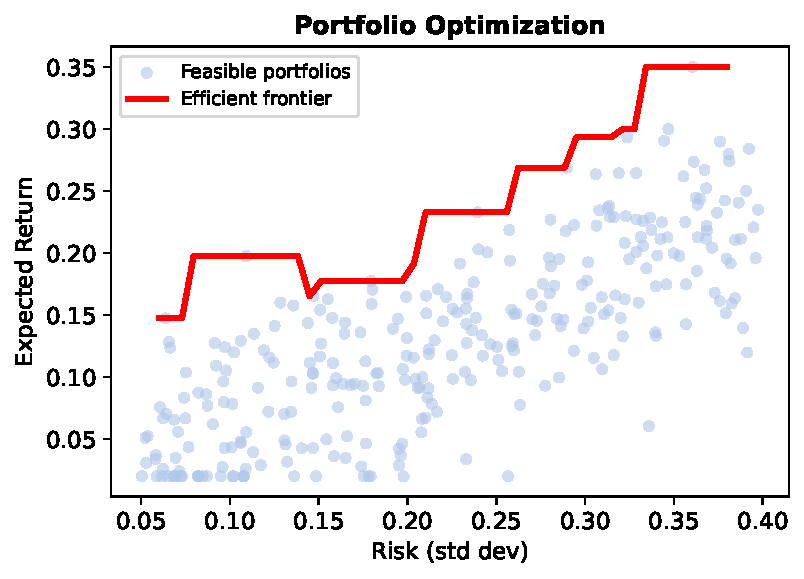
\includegraphics[width=\linewidth]{fig_portfolio}
  \end{columns}

  \framebreak

  \begin{columns}[T]
    \column{0.48\textwidth}
      \begin{block}{Medical Radiation Therapy Planning}
        In cancer radiotherapy, the goal is to deliver a prescribed radiation
        dose to the tumour while minimising collateral damage to surrounding
        healthy tissue.  The optimizer chooses the \emph{beam intensities}
        and \emph{beam angles} (collected in the design vector $\vx$).

        \medskip
        The objective is a risk measure over the spatial dose distribution ---
        for example, the Conditional Value-at-Risk (CVaR) of dose to critical
        organs.  Constraints require that the tumour receives at least the
        prescribed minimum dose everywhere.

        \medskip
        This is a large-scale linear or quadratic program, typically solved
        by interior-point methods (Chapter 11).
      \end{block}

      \vspace{0.4em}

      \begin{block}{Job Scheduling (Combinatorial Optimization)}
        Given $n$ jobs and $m$ machines, we want to assign jobs to machines
        to minimise the \emph{makespan} (the time until all jobs are finished).
        The number of possible orderings is $n!$ (n factorial), which grows
        explosively: for $n = 20$, that is over $2 \times 10^{18}$ possibilities.
        Exact methods are impractical for large $n$, so heuristics such as
        simulated annealing and genetic algorithms are used in practice.
      \end{block}

    \column{0.48\textwidth}
      \begin{alertblock}{Cross-Domain Summary}
        Despite their apparent differences, all five applications share
        the same mathematical skeleton: choose a vector of decision variables
        to minimise a scalar objective subject to constraints.
        \medskip
        \centering
        \begin{tabular}{lll}
          \toprule
          \textbf{Domain} & \textbf{Minimise} & \textbf{Variables} \\
          \midrule
          Aeronautics   & Drag             & Wing geometry \\
          Deep learning & Loss             & Network weights \\
          Finance       & Portfolio risk   & Asset fractions \\
          Medicine      & Organ dose       & Beam intensities \\
          Manufacturing & Makespan         & Job--machine assign.\ \\
          \bottomrule
        \end{tabular}
      \end{alertblock}
  \end{columns}

\end{frame}

%% ══════════════════════════════════════════════════════════════════════════
\section{Minima: Local vs.\ Global}
%% ══════════════════════════════════════════════════════════════════════════

\begin{frame}[allowframebreaks]{Types of Minima}

Not all ``low points'' of a function are equally desirable.  An algorithm
might converge to a point that is locally optimal but globally suboptimal.
This section defines precisely what we mean by local and global minima.

  \begin{columns}[T]
    \column{0.48\textwidth}

      \begin{block}{Global Minimum}
        A point $\vx^*$ is a \textbf{global minimum} of $f$ over $\mathcal{X}$ if
        \[
          f(\vx^*) \leq f(\vx) \quad \text{for all } \vx \in \mathcal{X}.
        \]
        In words: no other feasible point produces a smaller objective value.
        If the inequality is strict ($<$) for all $\vx \neq \vx^*$, then
        $\vx^*$ is the \emph{unique} global minimum.

        \medskip
        Finding the global minimum of a general non-convex function is
        NP-hard --- in the worst case, no algorithm can guarantee finding
        it without examining every point in $\mathcal{X}$.
      \end{block}

      \vspace{0.4em}

      \begin{block}{Local Minimum}
        A point $\vx^*$ is a \textbf{local minimum} if there exists a radius
        $\delta > 0$ (delta, read ``delta'', meaning a small positive number)
        such that
        \[
          f(\vx^*) \leq f(\vx)
          \quad \text{for all } \vx \in \mathcal{X} \text{ with }
          \|\vx - \vx^*\| < \delta.
        \]
        Here $\|\vx - \vx^*\|$ denotes the Euclidean distance between
        $\vx$ and $\vx^*$.  The condition says: within a ball of radius
        $\delta$ centred at $\vx^*$, no other feasible point is better.
        Outside this ball, there may well be points with smaller $f$ values.

        \medskip
        A \textbf{strong local minimum} satisfies the strict inequality
        $f(\vx^*) < f(\vx)$ for all $\vx \neq \vx^*$ within the ball.
        Every global minimum is also a local minimum, but the converse
        is false.
      \end{block}

    \column{0.50\textwidth}
      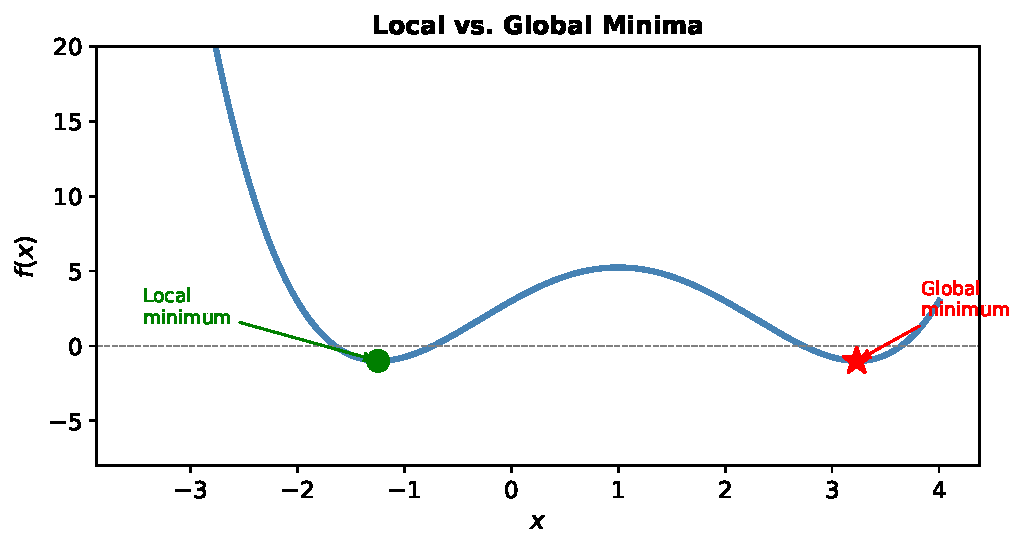
\includegraphics[width=\linewidth]{fig_local_global}
      \vspace{0.3em}
      \begin{exampleblock}{Concrete Numerical Example}
        Consider $f(x) = \tfrac{x^3}{3} - x$.

        \medskip
        Computing the derivative: $f'(x) = x^2 - 1$.
        Setting $f'(x) = 0$: $x^2 = 1$, so $x = \pm 1$.

        \medskip
        At $x = 1$: $f''(1) = 2 > 0$ --- this is a local minimum
        with $f(1) = \tfrac{1}{3} - 1 = -\tfrac{2}{3}$.

        \medskip
        At $x = -1$: $f''(-1) = -2 < 0$ --- this is a local maximum
        with $f(-1) = -\tfrac{1}{3} + 1 = \tfrac{2}{3}$.

        \medskip
        However, as $x \to -\infty$, $f(x) \to -\infty$, so the
        function is unbounded below and the local minimum at $x=1$
        is \textbf{not} a global minimum.
      \end{exampleblock}
  \end{columns}

  \framebreak

  \begin{block}{Classification of Stationary Points}
    \centering
    \begin{tabular}{llll}
      \toprule
      \textbf{Type} & \textbf{Condition on $f$} & \textbf{Uniqueness} & \textbf{Remark} \\
      \midrule
      Strong local min & $f(\vx^*) < f(\vx)$ for nearby $\vx \neq \vx^*$ & Locally unique & Most algorithms find these \\
      Weak local min   & $f(\vx^*) \leq f(\vx)$ for nearby $\vx$         & Plateau possible & Flat regions complicate search \\
      Global min       & $f(\vx^*) \leq f(\vx)$ for all $\vx \in \mathcal{X}$ & May or may not be unique & Hard to certify in general \\
      Saddle point     & $f'(\vx^*)=0$ but not a min or max              & N/A & Gradient descent can stall here \\
      \bottomrule
    \end{tabular}
  \end{block}

  \vspace{0.3em}

  \begin{alertblock}{Practical Implication: Most Algorithms Find Local Minima}
    The vast majority of practical optimization algorithms (gradient descent,
    Newton's method, quasi-Newton, conjugate gradients) are designed to
    find \emph{local} minima.  If the objective is non-convex, they may
    converge to a local minimum that is not globally optimal.

    \medskip
    Common strategies to escape local minima and search for a global minimum:
    \begin{itemize}
      \item \textbf{Multi-start}: run the algorithm from many random initial
        points and keep the best solution found.
      \item \textbf{Simulated annealing}: occasionally accept worse solutions
        with a probability that decreases over time, allowing the search
        to ``climb out'' of local basins.
      \item \textbf{Population methods} (genetic algorithms, particle swarm):
        maintain a diverse population of solutions to explore multiple regions.
      \item \textbf{Convex relaxation}: reformulate the problem to remove
        non-convexities and obtain a global bound.
    \end{itemize}
  \end{alertblock}

  \begin{columns}[T]
    \column{0.50\textwidth}
      \begin{exampleblock}{Exercise 1.1}
        \textbf{Question}: Give a function that has a local minimum that is
        not a global minimum.

        \medskip
        \textbf{Answer}: $f(x) = x^3/3 - x$.
        The local minimum at $x=1$ has value $f(1) = -2/3$, but
        $f(x) \to -\infty$ as $x \to -\infty$, so no global minimum exists.
      \end{exampleblock}

    \column{0.48\textwidth}
      \begin{exampleblock}{Exercise 1.2}
        \textbf{Question}: What is the minimum of $f(x) = x^3 - x$?

        \medskip
        \textbf{Answer}: No minimum exists.  As $x \to -\infty$,
        $f(x) \to -\infty$, so the function is unbounded below and has
        no global minimiser.
      \end{exampleblock}
  \end{columns}

\end{frame}

%% ══════════════════════════════════════════════════════════════════════════
\section{Optimality Conditions}
%% ══════════════════════════════════════════════════════════════════════════

\begin{frame}[allowframebreaks]{Optimality Conditions --- One Variable}

A key question is: how do we \emph{recognise} a minimum without exhaustively
checking every point?  The answer lies in optimality conditions --- mathematical
properties that every minimum must satisfy.  We begin with the one-dimensional
case for clarity, then generalise.

  \begin{block}{Setting: Unconstrained Univariate Minimisation}
    We consider the problem of minimising a smooth (continuously differentiable)
    function $f : \R \to \R$ without any constraints.  Our goal is to find
    conditions on $x^*$ that are \emph{necessary} for $x^*$ to be a local minimum.
  \end{block}

  \begin{columns}[T]
    \column{0.50\textwidth}

      \begin{alertblock}{First-Order Necessary Condition (FONC)}
        If $x^*$ is a local minimum of $f$, then
        \[
          f'(x^*) = 0.
        \]
        Here $f'(x^*)$ (f prime at x-star) is the derivative of $f$ evaluated
        at $x^*$.  A point where the derivative is zero is called a
        \textbf{stationary point}.

        \medskip
        \textbf{Why?} If $f'(x^*) > 0$, we could decrease $f$ by moving
        slightly to the left (decreasing $x$).  If $f'(x^*) < 0$, we could
        decrease $f$ by moving to the right.  Only when $f'(x^*) = 0$ is
        there no direction to improve.

        \medskip
        \textbf{Caution}: FONC is \emph{necessary but not sufficient}.
        A stationary point could be a maximum or a saddle (inflection) point.
      \end{alertblock}

      \vspace{0.4em}

      \begin{alertblock}{Second-Order Necessary Condition (SONC)}
        If $x^*$ is a local minimum of $f$, then
        \[
          f''(x^*) \geq 0.
        \]
        Here $f''(x^*)$ (f double-prime at x-star) is the second derivative,
        which measures the curvature of the function at $x^*$.
        A non-negative second derivative means the function is concave-up
        (bowl-shaped) at $x^*$, consistent with being at the bottom of a valley.
      \end{alertblock}

    \column{0.48\textwidth}

      \begin{block}{Sufficient Condition for a Strong Local Minimum}
        If both of the following hold:
        \[
          f'(x^*) = 0 \quad \text{and} \quad f''(x^*) > 0,
        \]
        then $x^*$ is a \textbf{strong local minimum}.  The strict
        inequality $f''(x^*) > 0$ ensures that the function curves
        upward, guaranteeing that nearby points have strictly larger
        $f$ values.
      \end{block}

      \vspace{0.4em}

      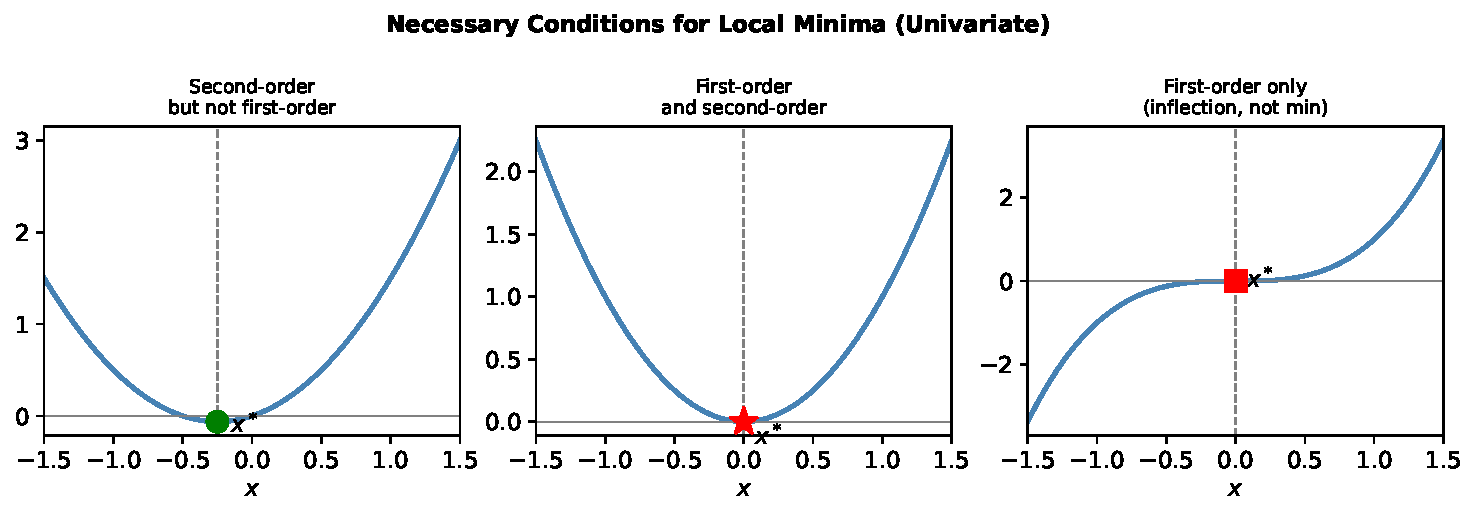
\includegraphics[width=\linewidth]{fig_optimality_1d}
  \end{columns}

  \framebreak

  \begin{block}{Derivation via Taylor Expansion}
    To see \emph{why} the FONC holds, we use a Taylor expansion.
    For a small step $h > 0$ (h, a positive real number), we have:
    \begin{align*}
      f(x^*+h) &= f(x^*) + h\,f'(x^*) + O(h^2), \tag{1.4}\\
      f(x^*-h) &= f(x^*) - h\,f'(x^*) + O(h^2). \tag{1.5}
    \end{align*}
    Here $O(h^2)$ (``big-O of h-squared'') denotes terms that shrink
    faster than $h$ as $h \to 0$ and can be neglected for small $h$.

    \medskip
    If $x^*$ is a local minimum, then for small enough $h$:
    \begin{align*}
      f(x^*+h) \geq f(x^*) &\implies h\,f'(x^*) \geq 0, \tag{1.6}\\
      f(x^*-h) \geq f(x^*) &\implies h\,f'(x^*) \leq 0. \tag{1.7}
    \end{align*}
    Combining (1.6) and (1.7): $h\,f'(x^*)$ must be both $\geq 0$ and
    $\leq 0$ simultaneously, which forces $f'(x^*) = 0$.
  \end{block}

  \begin{columns}[T]
    \column{0.50\textwidth}
      \begin{block}{Derivation of the SONC via Taylor Expansion}
        Using the FONC ($f'(x^*) = 0$), the second-order Taylor expansion gives:
        \begin{align*}
          f(x^*+h) &= f(x^*) + \underbrace{h\,f'(x^*)}_{=0}
                      + \frac{h^2}{2}\,f''(x^*) + O(h^3). \tag{1.9}
        \end{align*}
        If $x^*$ is a local minimum, $f(x^*+h) \geq f(x^*)$ for small $h$, so:
        \begin{align*}
          \frac{h^2}{2}\,f''(x^*) \geq 0 \implies f''(x^*) \geq 0, \tag{1.10}
        \end{align*}
        since $h^2 > 0$ for $h \neq 0$.
      \end{block}

    \column{0.48\textwidth}
      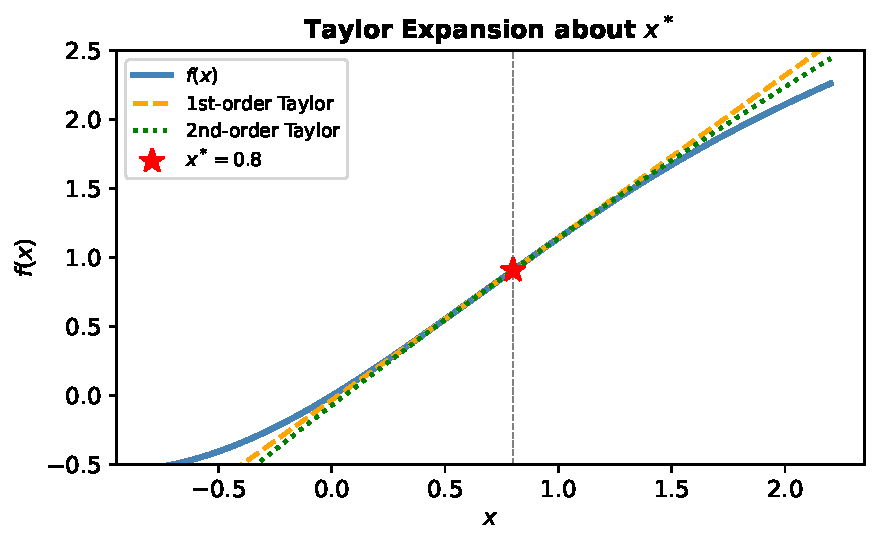
\includegraphics[width=\linewidth]{fig_taylor}
      \begin{block}{}
        \scriptsize The Taylor approximation $f(x^*+h) \approx f(x^*) +
        h f'(x^*) + \tfrac{h^2}{2} f''(x^*)$ becomes exact as $h \to 0$.
        The figure illustrates how well successive orders of the Taylor
        polynomial approximate $f$ near $x^*$.
      \end{block}
  \end{columns}

  \framebreak

  \begin{exampleblock}{Worked Example: Applying the Conditions to $f(x) = x^4 - 4x^2$}
    Let us verify the optimality conditions at the local minima of
    $f(x) = x^4 - 4x^2$.

    \medskip
    \textbf{Step 1 --- Find stationary points (FONC):}
    \[
      f'(x) = 4x^3 - 8x = 4x(x^2 - 2) = 0.
    \]
    Solutions: $x = 0,\; x = \sqrt{2} \approx 1.414,\; x = -\sqrt{2} \approx -1.414$.

    \medskip
    \textbf{Step 2 --- Apply the SONC at each stationary point:}
    \[
      f''(x) = 12x^2 - 8.
    \]
    \begin{itemize}
      \item At $x = 0$: $f''(0) = -8 < 0$ --- this is a \textbf{local maximum}.
      \item At $x = \sqrt{2}$: $f''(\sqrt{2}) = 12 \cdot 2 - 8 = 16 > 0$ ---
        \textbf{strong local minimum}, $f(\sqrt{2}) = 4 - 8 = -4$.
      \item At $x = -\sqrt{2}$: $f''(-\sqrt{2}) = 16 > 0$ ---
        \textbf{strong local minimum}, $f(-\sqrt{2}) = -4$.
    \end{itemize}

    \medskip
    Since $f(x) \to +\infty$ as $x \to \pm\infty$, both points $x = \pm\sqrt{2}$
    are also \textbf{global minima} with equal minimum value $-4$.
  \end{exampleblock}

\end{frame}

\begin{frame}[allowframebreaks]{Optimality Conditions --- Multiple Variables}

The one-dimensional conditions extend naturally to functions of $n$ variables,
but the derivative is replaced by the \emph{gradient} and the second derivative
is replaced by the \emph{Hessian matrix}.  These objects are central to the
rest of the book.

  \begin{columns}[T]
    \column{0.52\textwidth}

      \begin{alertblock}{First-Order Necessary Condition (Multivariate FONC)}
        If $\vx^*$ is a local minimum of $f : \R^n \to \R$, then
        \[
          \grad f(\vx^*) = \mathbf{0}.
        \]
        Here $\grad$ (nabla, also written $\nabla$, meaning ``gradient'' or
        ``del'') denotes the vector of partial derivatives:
        \[
          \grad f(\vx) = \left[\frac{\partial f}{\partial x_1},\;
          \frac{\partial f}{\partial x_2},\; \ldots,\;
          \frac{\partial f}{\partial x_n}\right]^\top.
        \]
        The notation $\partial f / \partial x_i$ (partial derivative of $f$
        with respect to $x_i$) measures how $f$ changes when only $x_i$
        changes and all other variables are held fixed.

        \medskip
        The condition $\grad f(\vx^*) = \mathbf{0}$ (gradient equals the zero
        vector) means that the function has no direction in which it can be
        immediately decreased: all partial derivatives are zero simultaneously.
      \end{alertblock}

    \column{0.46\textwidth}

      \begin{alertblock}{Second-Order Necessary Condition (Multivariate SONC)}
        If $\vx^*$ is a local minimum, then the \textbf{Hessian matrix}
        $\hess f(\vx^*)$ must be \emph{positive semidefinite}:
        \[
          \hess f(\vx^*) \succeq 0.
        \]
        The symbol $\succeq 0$ (succeeds or equals zero) means positive
        semidefinite: every eigenvalue is $\geq 0$.  The Hessian is the
        $n \times n$ matrix of second-order partial derivatives:
        \[
          [\hess f(\vx)]_{ij} = \frac{\partial^2 f}{\partial x_i \,\partial x_j}.
        \]
        Intuitively, the Hessian plays the role of curvature in
        multiple dimensions: it tells us how the function bends in
        each direction.
      \end{alertblock}

  \end{columns}

  \framebreak

  \begin{block}{Three Cases at a Stationary Point ($\grad f = \mathbf{0}$)}
    Once we find a stationary point $\vx^*$ (satisfying FONC), the Hessian
    tells us what kind of stationary point it is:
    \begin{enumerate}
      \item \textbf{Local minimum (bowl shape)}: $\hess f(\vx^*) \succ 0$
        (positive definite --- all eigenvalues $> 0$).  The function curves
        upward in every direction.
      \item \textbf{Local maximum (hill shape)}: $\hess f(\vx^*) \prec 0$
        (negative definite --- all eigenvalues $< 0$).  The function curves
        downward in every direction.
      \item \textbf{Saddle point}: $\hess f(\vx^*)$ is indefinite (some
        eigenvalues positive, some negative).  The function curves upward in
        some directions and downward in others --- like the surface of a
        horse saddle.  This is \emph{not} a local minimum.
    \end{enumerate}
    \vspace{0.3em}
    \centering
    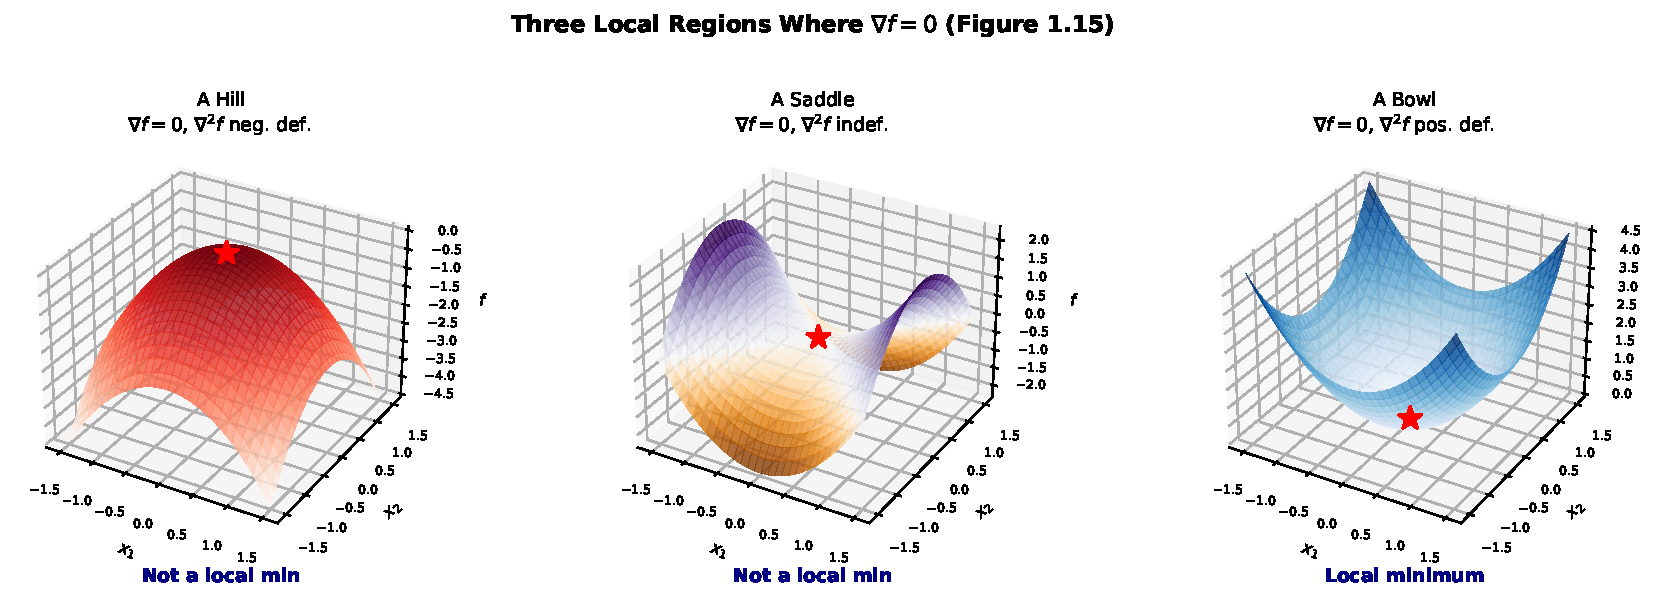
\includegraphics[width=0.55\linewidth]{fig_multivariate_regions}
  \end{block}

  \framebreak

  \begin{exampleblock}{Worked Example: The Rosenbrock Function}
    The \textbf{Rosenbrock function} is a famous benchmark for optimization
    algorithms because its minimum sits at the bottom of a long, narrow,
    curved valley that is very hard to navigate:
    \[
      f(\vx) = (1 - x_1)^2 + 5(x_2 - x_1^2)^2.
    \]
    We verify that $\vx^* = (1, 1)$ satisfies both FONC and SONC.

    \medskip
    \textbf{Step 1 --- Compute the gradient:}
    \[
      \frac{\partial f}{\partial x_1} = 2(10x_1^3 - 10x_1 x_2 + x_1 - 1), \qquad
      \frac{\partial f}{\partial x_2} = 10(x_2 - x_1^2).
    \]
    At $(1, 1)$: both partials equal $0$.  So $\grad f(1,1) = \mathbf{0}$. \checkmark

    \medskip
    \textbf{Step 2 --- Compute the Hessian:}
    \[
      \hess f(\vx) = \begin{bmatrix}
        -20(x_2 - x_1^2) + 40x_1^2 + 2 & -20x_1 \\
        -20x_1 & 10
      \end{bmatrix}.
    \]
    At $(1,1)$: substituting $x_1 = x_2 = 1$ gives $x_2 - x_1^2 = 0$, so
    \[
      \hess f(1,1) = \begin{bmatrix} 40 + 2 & -20 \\ -20 & 10 \end{bmatrix}
      = \begin{bmatrix} 42 & -20 \\ -20 & 10 \end{bmatrix}.
    \]
    \textbf{Step 3 --- Check positive definiteness:}
    For a $2 \times 2$ matrix, it is positive definite if and only if both the
    $(1,1)$ entry and the determinant are positive.
    \[
      \text{det}(\hess f) = 42 \times 10 - (-20)^2 = 420 - 400 = 20 > 0. \checkmark
    \]
    The leading entry $42 > 0$ and $\text{det} = 20 > 0$, so $\hess f(1,1)$ is
    positive definite, confirming that $(1,1)$ is a \textbf{strong local minimum}
    (in fact the unique global minimum, since $f(1,1) = 0$).
  \end{exampleblock}

  \framebreak

  \begin{columns}[T]
    \column{0.53\textwidth}
      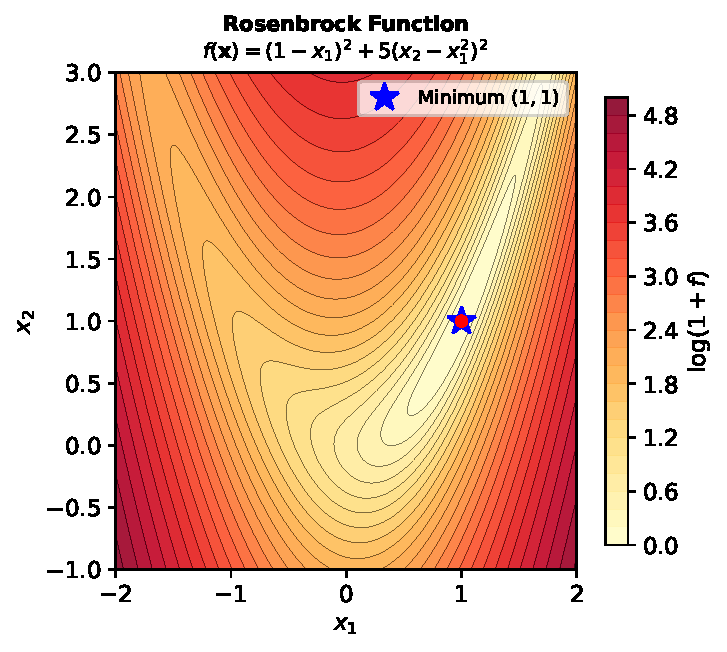
\includegraphics[width=\linewidth]{fig_rosenbrock}
    \column{0.45\textwidth}
      \begin{block}{Reading the Rosenbrock Contour Plot}
        A contour plot shows lines along which the function value is constant
        (like elevation contours on a topographic map).  In the Rosenbrock
        plot, the contours form an elongated banana-shaped valley.

        \medskip
        The minimum $(1,1)$ sits at the centre of the tightest contours.
        The valley is extremely narrow in one direction and almost flat
        in the other --- this is why simple gradient descent struggles:
        a step that is large enough to make progress along the valley
        is too large to stay within it.
      \end{block}
      \begin{exampleblock}{Saddle Point Comparison}
        For $f(x_1, x_2) = x_1^2 - x_2^2$:
        \begin{itemize}
          \item $\grad f = [2x_1,\; -2x_2]^\top = \mathbf{0}$ at the origin.
          \item $\hess f = \text{diag}(2, -2)$ --- eigenvalues $+2$ and $-2$
            --- indefinite.
          \item Conclusion: the origin is a \textbf{saddle point}, not a minimum.
        \end{itemize}
      \end{exampleblock}
  \end{columns}

\end{frame}

\begin{frame}[fragile]{Optimality Conditions --- Python Verification}

The following Python code computes the gradient and Hessian of the Rosenbrock
function numerically and verifies that $(1, 1)$ satisfies both FONC and SONC.
This pattern --- compute gradient, compute Hessian, check eigenvalues ---
is a standard verification workflow.

  \begin{columns}[T]
    \column{0.54\textwidth}
      \begin{lstlisting}[style=pycode,caption={Checking optimality conditions for the Rosenbrock function}]
import numpy as np

def rosenbrock(x):
    """f(x) = (1-x1)^2 + 5*(x2-x1^2)^2"""
    return (1 - x[0])**2 + 5*(x[1] - x[0]**2)**2

def grad_rosenbrock(x):
    """Gradient vector [df/dx1, df/dx2]"""
    x1, x2 = x
    df_dx1 = 2*(10*x1**3 - 10*x1*x2 + x1 - 1)
    df_dx2 = 10*(x2 - x1**2)
    return np.array([df_dx1, df_dx2])

def hess_rosenbrock(x):
    """2x2 Hessian matrix of second derivatives"""
    x1, x2 = x
    h11 = -20*(x2 - x1**2) + 40*x1**2 + 2
    h12 = -20*x1
    h22 = 10
    return np.array([[h11, h12], [h12, h22]])

xstar = np.array([1.0, 1.0])
g = grad_rosenbrock(xstar)
H = hess_rosenbrock(xstar)
# eigvalsh assumes H is symmetric (it is, by Clairaut's theorem)
eigs = np.linalg.eigvalsh(H)

print("Gradient:", g)         # should be [0. 0.]
print("Hessian:\n", H)        # [[42 -20][-20 10]]
print("Eigenvalues:", eigs)   # should be > 0 (positive definite)
print("FONC satisfied:", np.allclose(g, 0))
print("SONC satisfied:", np.all(eigs >= 0))
      \end{lstlisting}

    \column{0.44\textwidth}
      \begin{block}{Expected Output}
        \texttt{Gradient: [0. 0.]}\\[2pt]
        \texttt{Hessian:}\\
        \texttt{\ [[42. -20.]}\\
        \texttt{\ \ [-20.  10.]]}\\[2pt]
        \texttt{Eigenvalues: [2.0, 50.0]}\\
        \texttt{(both positive)}\\[4pt]
        \texttt{FONC satisfied: True}\\
        \texttt{SONC satisfied: True}
      \end{block}
      \begin{alertblock}{Conclusion}
        Both conditions are satisfied at $\vx^* = (1, 1)$, confirming
        it is a strong local minimum.  Since it is also the unique global
        minimum of the Rosenbrock function, $f(\vx^*) = 0$.

        \medskip
        Note: \texttt{np.linalg.eigvalsh} is used instead of \texttt{eigvals}
        because $H$ is symmetric (the Hessian of a smooth function is always
        symmetric, by Clairaut's theorem), and \texttt{eigvalsh} exploits
        symmetry for numerical stability.
      \end{alertblock}
  \end{columns}

\end{frame}

\begin{frame}[fragile]{Surface and Contour Visualisation}

Visualising the objective function as a 3-D surface and a 2-D contour plot
helps develop geometric intuition about where minima, maxima, and saddle
points are located.  The code below plots the saddle function
$f(x_1, x_2) = x_1^2 - x_2^2$.

  \begin{columns}[T]
    \column{0.54\textwidth}
      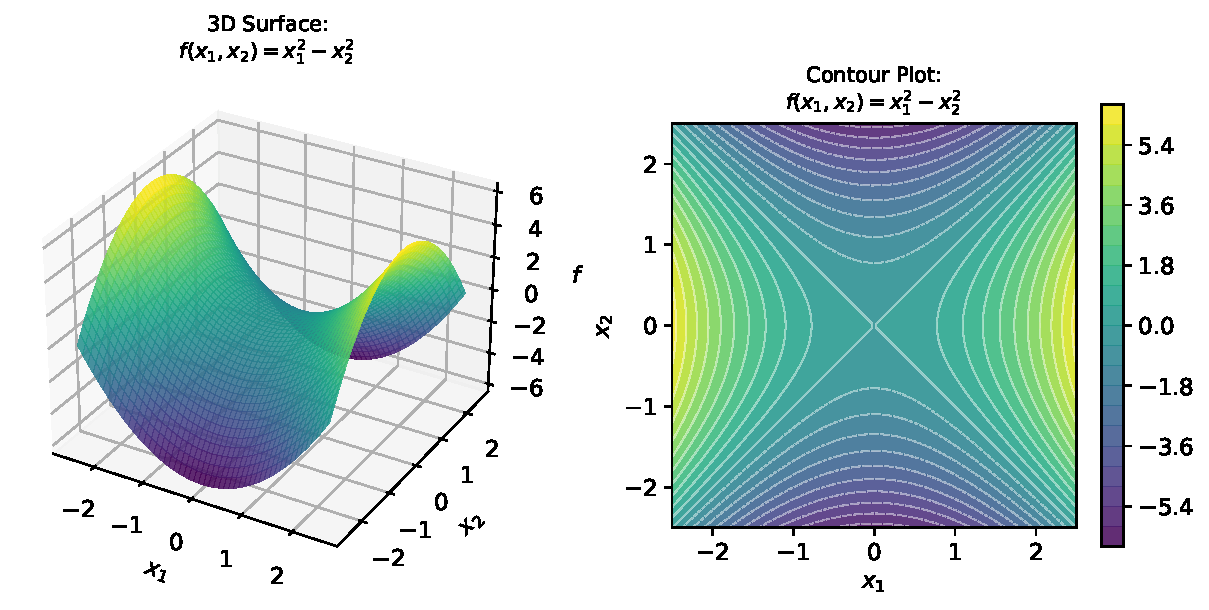
\includegraphics[width=\linewidth]{fig_surface_contour}
    \column{0.44\textwidth}
      \begin{lstlisting}[style=pycode,caption={3D surface + contour plot}]
import numpy as np
import matplotlib.pyplot as plt
from mpl_toolkits.mplot3d import Axes3D

x1 = np.linspace(-2.5, 2.5, 100)
x2 = np.linspace(-2.5, 2.5, 100)
X1, X2 = np.meshgrid(x1, x2)
Z = X1**2 - X2**2   # saddle function

fig = plt.figure(figsize=(10, 4))

# 3-D surface plot
ax3d = fig.add_subplot(121, projection='3d')
ax3d.plot_surface(X1, X2, Z, cmap='viridis')
ax3d.set_xlabel('$x_1$')
ax3d.set_ylabel('$x_2$')
ax3d.set_title('Surface')

# 2-D filled contour plot
ax2d = fig.add_subplot(122)
ax2d.contourf(X1, X2, Z, 20, cmap='viridis')
ax2d.set_xlabel('$x_1$')
ax2d.set_ylabel('$x_2$')
ax2d.set_title('Contour (top view)')

plt.tight_layout()
plt.savefig('fig_surface_contour.pdf')
      \end{lstlisting}
      \begin{block}{}
        \scriptsize The 3-D surface (left) shows the saddle shape of
        $f = x_1^2 - x_2^2$: curves up along $x_1$ and down along $x_2$.
        The 2-D contour (right) shows this as a top-down view, with colour
        encoding $f$ values.  The origin is a saddle point --- not a minimum.
      \end{block}
  \end{columns}

\end{frame}

%% ══════════════════════════════════════════════════════════════════════════
\section{Overview of the Book}
%% ══════════════════════════════════════════════════════════════════════════

\begin{frame}[allowframebreaks]{Overview of the Book}

This book is organised around the structure of optimization problems:
we begin with the simplest case (one-dimensional, unconstrained, smooth)
and progressively add complexity (higher dimensions, constraints, noise,
multiple objectives).  Understanding where each chapter fits in the overall
roadmap will help you navigate the material.

  \begin{columns}[T]
    \column{0.50\textwidth}
      \begin{block}{Part I: Foundations (Chapters 1--4)}
        \begin{description}
          \item[Ch.\ 1] \textbf{Introduction} (this chapter): formulation,
            history, applications, and optimality conditions.
          \item[Ch.\ 2] \textbf{Derivatives and Gradients}: how to compute
            derivatives analytically, numerically (finite differences), and
            exactly (automatic differentiation).
          \item[Ch.\ 3] \textbf{Bracketing}: finding an interval that contains
            a minimum for one-dimensional problems.
          \item[Ch.\ 4] \textbf{Local Descent}: the general descent framework
            and derivative-free methods (Nelder--Mead, coordinate descent).
        \end{description}
      \end{block}

      \vspace{0.3em}

      \begin{block}{Part II: Gradient-Based Methods (Chapters 5--9)}
        \begin{description}
          \item[Ch.\ 5] \textbf{First-Order Methods}: gradient descent,
            momentum, subgradient methods.
          \item[Ch.\ 6] \textbf{Second-Order Methods}: Newton's method,
            quasi-Newton (BFGS, L-BFGS).
          \item[Ch.\ 7] \textbf{Conjugate Direction Methods}: avoids
            redundant search directions; more efficient than gradient descent.
          \item[Ch.\ 8] \textbf{Stochastic Methods}: SGD, AdaGrad, Adam
            for large-scale and noisy settings.
          \item[Ch.\ 9] \textbf{Noisy Objectives}: methods for objectives
            corrupted by measurement noise.
        \end{description}
      \end{block}

    \column{0.48\textwidth}
      \begin{block}{Part III: Constrained and Specialised (Chapters 10--16)}
        \begin{description}
          \item[Ch.\ 10] \textbf{Constraints}: KKT conditions, penalty methods,
            augmented Lagrangian, active-set methods.
          \item[Ch.\ 11] \textbf{Linear Programming}: Simplex algorithm,
            interior-point methods.
          \item[Ch.\ 12] \textbf{Network Flow}: min-cost flow, shortest paths.
          \item[Ch.\ 13] \textbf{Sampling Plans}: space-filling designs for
            expensive black-box functions.
          \item[Ch.\ 14] \textbf{Surrogate Models}: fit a cheap model to
            replace expensive evaluations.
        \end{description}
      \end{block}

      \begin{block}{Part IV: Advanced Topics (Chapters 17--24)}
        \begin{description}
          \item[Ch.\ 17] \textbf{Surrogate Optimization}: Bayesian optimisation
            with acquisition functions (expected improvement).
          \item[Ch.\ 20] \textbf{Uncertainty}: robust and probabilistic
            optimization.
          \item[Ch.\ 21] \textbf{Multi-Objective}: Pareto fronts,
            scalarisation, NSGA-II.
          \item[Ch.\ 23] \textbf{Expression Optimization}: symbolic regression.
          \item[Ch.\ 24] \textbf{Multidisciplinary Design}: coupling multiple
            engineering disciplines.
        \end{description}
      \end{block}
  \end{columns}

  \framebreak

  \begin{columns}[T]
    \column{0.50\textwidth}
      \begin{block}{The Progression from Simple to Complex}
        Chapters 5--9 all assume the objective is smooth and unconstrained
        (or only box-constrained).  They differ in \emph{what information
        about $f$ they use}:

        \medskip
        \textbf{Chapter 5} uses only the gradient $\grad f$ (first-order
        information).  This is sufficient to find a descent direction, but
        convergence can be slow near the minimum because the gradient
        gives no information about curvature.

        \medskip
        \textbf{Chapter 6} adds the Hessian $\hess f$ (second-order
        information), allowing Newton's method to take much more accurate
        steps.  The cost is computing and factorising the $n \times n$ Hessian,
        which is expensive when $n$ is large.

        \medskip
        \textbf{Chapter 7} uses conjugate directions, which accumulate
        information from previous steps to avoid searching in the same
        direction twice.  This is especially effective for quadratic objectives.

        \medskip
        \textbf{Chapters 8--9} handle the stochastic setting where $\grad f$
        is not available exactly but can be estimated from random samples.
        This is the regime of modern deep learning.
      \end{block}

    \column{0.48\textwidth}
      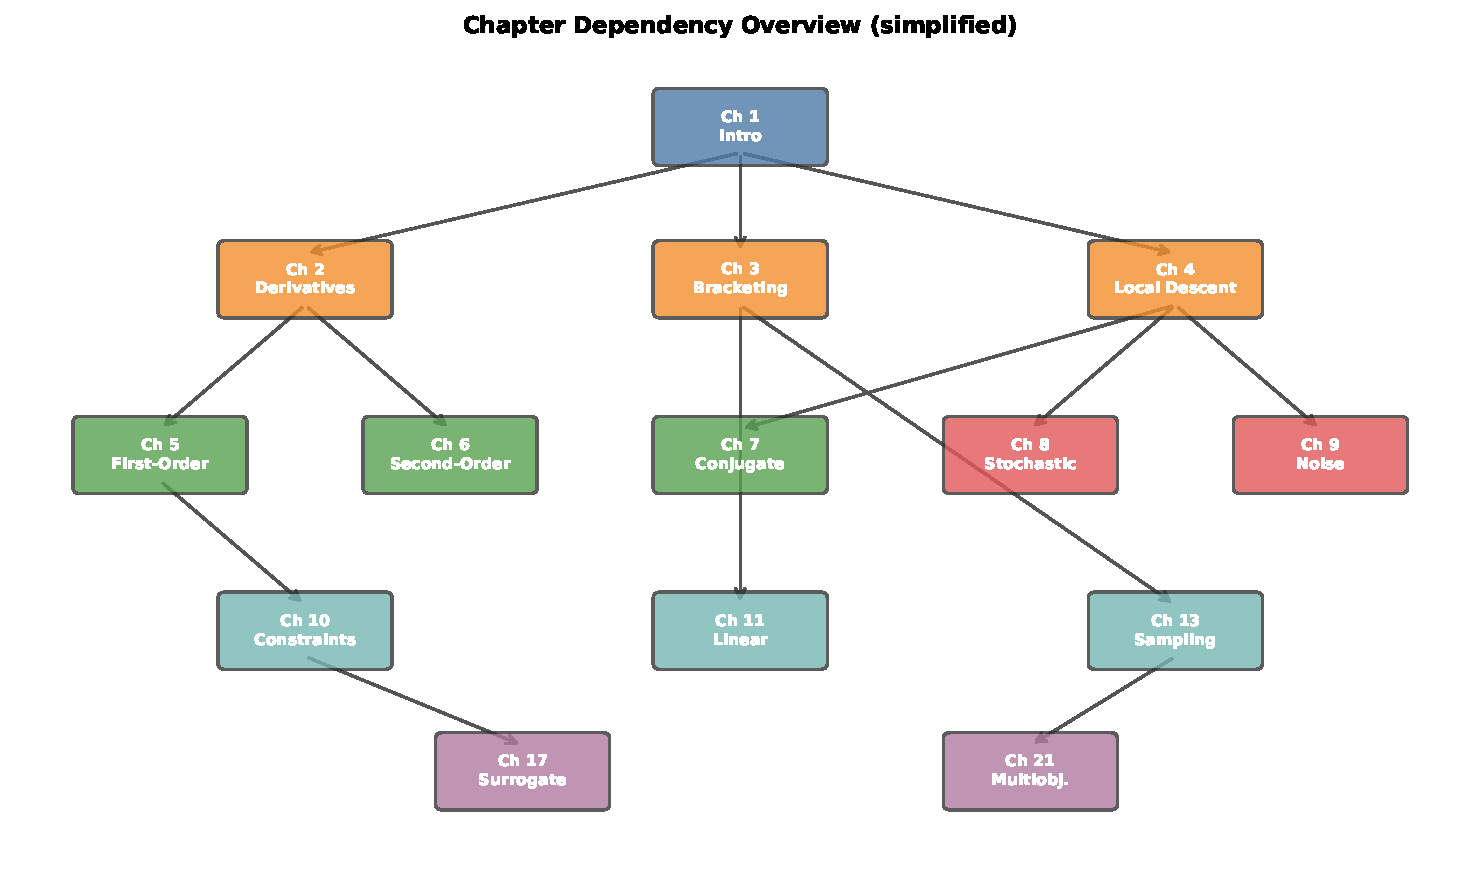
\includegraphics[width=\linewidth]{fig_chapter_tree}
      \vspace{0.3em}
      \begin{block}{}
        \scriptsize The chapter dependency graph shows which earlier chapters
        are prerequisites for each later chapter.  Arrows indicate ``should
        be read before.''  Chapters 1--4 form the mandatory foundation for
        all subsequent material.
      \end{block}
  \end{columns}

  \framebreak

  \begin{block}{When Gradients Are Unavailable: Surrogate and Bayesian Methods}
    Many real engineering problems do not provide gradients.  Either the
    objective is computed by a legacy simulator that outputs only a scalar,
    or the function is stochastic and gradients are too noisy to be useful.
    In these cases, we must rely on \emph{function values alone}.

    \medskip
    \textbf{Surrogate models} (Chapter 14): fit a computationally cheap model
    (such as a Gaussian process or polynomial regression) to the observed
    function values, then optimise the cheap model instead.

    \medskip
    \textbf{Bayesian optimisation} (Chapter 17): maintain a probabilistic
    belief (posterior distribution) over the function $f$, and choose the
    next evaluation point by maximising an \emph{acquisition function} that
    balances exploitation (evaluating near the current best estimate) with
    exploration (reducing uncertainty in unexplored regions).
  \end{block}

  \begin{exampleblock}{Algorithm Families at a Glance}
    \centering
    \begin{tabular}{llll}
      \toprule
      \textbf{Family} & \textbf{Information used} & \textbf{Key chapter(s)} & \textbf{Typical $n$} \\
      \midrule
      First-order gradient   & $\grad f$           & 5, 6         & Any \\
      Second-order (Newton)  & $\hess f$           & 6            & Small--medium \\
      Conjugate direction    & History of $\grad f$ & 7           & Medium \\
      Stochastic gradient    & Noisy $\grad f$     & 8, 9         & Very large \\
      Evolutionary           & $f$ values only     & 14           & Small--medium \\
      Bayesian optimisation  & Posterior over $f$  & 17           & Very small \\
      \bottomrule
    \end{tabular}
  \end{exampleblock}

\end{frame}

%% ══════════════════════════════════════════════════════════════════════════
\section{Summary \& Exercises}
%% ══════════════════════════════════════════════════════════════════════════

\begin{frame}[allowframebreaks]{Summary of Chapter 1}

Chapter 1 introduced the fundamental concepts that underpin every topic in
this book.  Before proceeding to the algorithms, make sure you can state and
apply each of the following ideas.

  \begin{columns}[T]
    \column{0.52\textwidth}
      \begin{block}{Core Concepts}
        \begin{enumerate}
          \item \textbf{What is optimization?}  The process of choosing a
            design vector $\vx$ from a feasible set $\mathcal{X}$ to
            minimise (or maximise) an objective function $f(\vx)$.

          \item \textbf{Standard form}: every problem can be written as
            \[
              \min_{\vx \in \mathcal{X}} f(\vx)
              \quad \text{subject to constraints.}
            \]

          \item \textbf{Local minimum}: a point where $f(\vx^*) \leq f(\vx)$
            for all nearby $\vx$.  Global minimum: this holds for \emph{all}
            feasible $\vx$.

          \item \textbf{First-Order Necessary Condition (FONC)}:
            $\grad f(\vx^*) = \mathbf{0}$.  Zero gradient is necessary but
            not sufficient for a minimum.

          \item \textbf{Second-Order Necessary Condition (SONC)}:
            $\hess f(\vx^*) \succeq 0$.  Positive semidefinite Hessian rules
            out local maxima.

          \item \textbf{Sufficient condition} for a strong local minimum:
            $\grad f = \mathbf{0}$ \emph{and} $\hess f \succ 0$ (positive definite).

          \item \textbf{No Free Lunch}: no single algorithm is best for all
            problems.  Algorithm selection depends on problem structure.
        \end{enumerate}
      \end{block}

    \column{0.46\textwidth}
      \begin{alertblock}{Core Formulas to Memorise}
        \[
          \text{FONC (1-D):}\quad f'(x^*)=0
        \]
        \[
          \text{FONC (n-D):}\quad \grad f(\vx^*)=\mathbf{0}
        \]
        \[
          \text{SONC (1-D):}\quad f''(x^*)\geq 0
        \]
        \[
          \text{SONC (n-D):}\quad \hess f(\vx^*)\succeq 0
        \]
        \[
          \text{Sufficient:}\quad f'(x^*)=0,\; f''(x^*)>0
        \]
      \end{alertblock}

      \vspace{0.4em}

      \begin{block}{Applications Span Many Fields}
        The same mathematical framework applies to:
        aerospace engineering (aerodynamic drag minimisation),
        machine learning (loss minimisation over neural network weights),
        quantitative finance (portfolio risk minimisation),
        medicine (radiation dose planning),
        and manufacturing (job scheduling).
      \end{block}
  \end{columns}

\end{frame}

\begin{frame}[allowframebreaks]{Exercises (with Full Solutions)}

The following exercises are drawn from the textbook.  Work through them
yourself before reading the solutions --- the process of attempting a
problem is more valuable than simply reading the answer.

  \begin{block}{Exercise 1.1}
    \textbf{Question}: Give an example of a function that has a local minimum
    that is not a global minimum.

    \medskip
    \textbf{Solution}: Consider $f(x) = \tfrac{x^3}{3} - x$.
    \begin{itemize}
      \item $f'(x) = x^2 - 1 = 0$ gives stationary points at $x = \pm 1$.
      \item $f''(1) = 2 > 0$, confirming $x = 1$ is a local minimum with
        $f(1) = \tfrac{1}{3} - 1 = -\tfrac{2}{3}$.
      \item As $x \to -\infty$, $f(x) = \tfrac{x^3}{3} - x \to -\infty$,
        so the function is unbounded below.  Therefore $x = 1$ cannot be
        a global minimum.
    \end{itemize}
  \end{block}

  \begin{block}{Exercise 1.2}
    \textbf{Question}: What is the minimum of $f(x) = x^3 - x$?

    \medskip
    \textbf{Solution}: No minimum exists.  As $x \to -\infty$,
    $x^3$ dominates and $f(x) \to -\infty$, so $f$ has no lower bound
    and therefore no global minimiser.
  \end{block}

  \begin{block}{Exercise 1.3}
    \textbf{Question}: Give a function that is bounded below but has no
    global optimum on $\mathcal{X} = [0, 1]$.

    \medskip
    \textbf{Solution}: Define
    \[
      f(x) = \begin{cases} |x| & \text{if } x \neq 0 \\ 1 & \text{if } x = 0 \end{cases}.
    \]
    This function satisfies $f(x) \geq 0$ for all $x$ (bounded below by $0$).
    The infimum is $\inf_{x \in [0,1]} f(x) = 0$, but this infimum is not
    attained: at $x = 0$ the function value is $1$, not $0$, and for any
    $x > 0$ we have $f(x) = x > 0$.  So there is no point in $[0,1]$
    where $f$ achieves its infimum.
  \end{block}

  \framebreak

  \begin{block}{Exercise 1.4}
    \textbf{Question}: What are the minima and minimizers of $f(x) = \sin(x)$?

    \medskip
    \textbf{Solution}: The function $\sin(x)$ is periodic with period $2\pi$
    (2 pi, approximately 6.28).  Its minimum value is $-1$, attained whenever
    $x = \tfrac{3}{2}\pi + 2\pi k$ for any integer $k$ (since $\sin(3\pi/2) = -1$).
    There are infinitely many global minimizers, all equally optimal.
  \end{block}

  \begin{block}{Exercise 1.5}
    \textbf{Question}: Does the FONC $f'(x) = 0$ necessarily hold at the
    optimal solution of a \emph{constrained} problem?

    \medskip
    \textbf{Solution}: \textbf{No.}  Consider $\min_{x} f(x) = x$
    subject to $x \geq 1$.  The optimal solution is $x^* = 1$ (the
    smallest feasible value), but $f'(1) = 1 \neq 0$.

    \medskip
    This shows that for constrained problems, the unconstrained FONC
    no longer applies.  The correct conditions are the
    \textbf{KKT (Karush--Kuhn--Tucker) conditions} (Chapter 10),
    which account for the fact that the optimizer is ``pushing against''
    a constraint boundary.
  \end{block}

  \begin{block}{Exercise 1.6}
    \textbf{Question}: How many minima does $f(x, y) = x^2 + y$ have,
    subject to the constraints $x > y \geq 1$?

    \medskip
    \textbf{Solution}: \textbf{None.}  The constraint $x > y$ is a
    \emph{strict} inequality, so the boundary $x = y$ is excluded from
    the feasible set.  As we let $x \to y^+$ (x approaches y from above)
    and $y \to 1^+$ (y approaches 1 from above), $f(x, y) \to 1 + 1 = 2$,
    but we can never actually attain $f = 2$ because the boundary is excluded.
    Therefore the infimum (greatest lower bound) of $f$ over the feasible set
    is $2$, but no minimiser exists.
  \end{block}

  \framebreak

  \begin{block}{Exercise 1.7}
    \textbf{Question}: How many inflection points does $f(x) = x^3 - 10$ have?

    \medskip
    \textbf{Solution}: An inflection point is a point where the second
    derivative changes sign.  Computing:
    \[
      f'(x) = 3x^2, \qquad f''(x) = 6x.
    \]
    Setting $f''(x) = 6x = 0$ gives $x = 0$.  For $x < 0$, $f''(x) < 0$
    (concave down); for $x > 0$, $f''(x) > 0$ (concave up).  Since the
    sign of $f''$ changes at $x = 0$, there is exactly \textbf{one} inflection
    point, at $x = 0$.

    \medskip
    Note: the $-10$ is just a vertical shift and does not affect the shape
    or the location of the inflection point.
  \end{block}

  \vspace{0.5em}

  \begin{exampleblock}{Study Tips for Chapter 1}
    \begin{itemize}
      \item Always check \emph{both} FONC \emph{and} SONC when identifying
        a minimum.  FONC alone is not sufficient --- a stationary point could
        be a maximum or saddle.

      \item For constrained problems, the unconstrained FONC does not apply.
        The correct framework is the KKT conditions, introduced in Chapter 10.
        Keep this in mind when working on applied problems.

      \item In Python, \texttt{scipy.optimize.minimize} is your go-to solver.
        Use \texttt{method='L-BFGS-B'} for unconstrained or box-constrained
        problems, and \texttt{method='SLSQP'} when you have general inequality
        or equality constraints.

      \item Draw the function before running an algorithm.  For one- and
        two-dimensional problems, plotting the objective and feasible set
        often reveals whether local minima exist and where the global minimum
        is likely to be.
    \end{itemize}
  \end{exampleblock}

\end{frame}

%% ── Final slide ───────────────────────────────────────────────────────────
\begin{frame}{End of Chapter 1}
  \begin{center}
    \LARGE\textbf{Chapter 1: Introduction}\\[1em]
    \large Algorithms for Optimization\\[0.5em]
    \normalsize Kochenderfer \& Wheeler, 2nd Ed.\ (2026)
  \end{center}
  \vspace{1em}
  \begin{columns}[c]
    \column{0.48\textwidth}
      \begin{block}{What We Covered in This Chapter}
        \begin{itemize}
          \item A brief history of optimization from ancient geometry
            to modern deep learning.
          \item The five-step engineering optimization process.
          \item Standard mathematical formulation: objective, constraints,
            feasible set.
          \item Applications across aerospace, machine learning,
            finance, medicine, and manufacturing.
          \item Local vs.\ global minima, and why the difference matters.
          \item Optimality conditions: FONC ($\grad f = \mathbf{0}$)
            and SONC ($\hess f \succeq 0$) for both one and many variables.
          \item Roadmap of the book's 24 chapters.
        \end{itemize}
      \end{block}
    \column{0.48\textwidth}
      \begin{block}{Up Next: Chapter 2 --- Derivatives and Gradients}
        Before we can use gradient-based algorithms, we need reliable
        methods to compute derivatives.  Chapter 2 covers:
        \begin{itemize}
          \item Finite difference approximations (forward, central, backward).
          \item The complex-step method for high-accuracy numerical derivatives.
          \item Automatic differentiation (forward and reverse modes) ---
            the engine behind modern deep learning frameworks.
          \item Directional derivatives and their role in line search.
        \end{itemize}
      \end{block}
  \end{columns}
\end{frame}

\end{document}
